\chapter{Gaussian elimination}

\section{Introduction}
Gaussian elimination (also known as row reduction) is an algorithm for solving systems of linear equations. It is usually understood as a sequence of operations performed on the corresponding matrix of coefficients. \\
The fundamental idea is to add multiples of one equation to the others in order to eliminate a variable and to continue this process until only one variable is left. Once this final variable is determined, its value is substituted back into the other equations in order to evaluate the remaining unknowns. This method, characterized by step$-$by$-$step  elimination of the variables, is called Gaussian elimination.\\
$\begin{bmatrix}
1&3& \\
2&1&				
\end{bmatrix}$
$\begin{bmatrix}
x \\
y				
\end{bmatrix}$
=
$\begin{bmatrix}
3 \\
5				
\end{bmatrix}$\\

$\begin{matrix}
1x+3y = 3 \\
2x+1y = 5				
\end{matrix}$\\

Multiply row 1 by 2 and subtract from row 2 \\
$\begin{matrix}
1x+3y = 3 \\
5y = 1				
\end{matrix}$\\
$\begin{matrix}
x = 12/5 \\
y = 1/5				
\end{matrix}$
\section{C++ implementation}
The C++ implementation as below:
\begin{lstlisting}[language=C, caption=Gauss elimination in C++]
	void Gauss_elmination_cpu(float a[], float d[], int n) {
	int i, j, k, temp;
	//********* Forward elimination process**************//
	for (int i = 0; i < n - 1; i++) {
		for (int k = i + 1; k < n; k++) {
			float c = a[k * (n + 1) + i] / a[i * (n + 1) + i];
			for (int j = i; j <= n; j++) {
				a[k * (n + 1) + j] = a[k * (n + 1) + j] - (c * a[i * (n + 1) + j]);
			}
		}
	}
    //***************** Backward Substitution method****************//
	for (i = n - 1; i >= 0; i--){
		d[i] = a[i * (n + 1) + n];
		for (int j = i + 1; j < n; j++) {
			if (j != i) {
				d[i] = d[i] - a[i * (n + 1) + j] * d[j];
			}
		}
		d[i] = d[i] / a[i * (n + 1) + i];
	}
}
\end{lstlisting}
\textbf{Forward elimination:} reduction to row echelon form. Using it one can tell whether there are no solutions, or unique solution, or infinitely many solutions.\\
\textbf{Back substitution:} further reduction to reduced row echelon form.\\
In this code, We have i is the row number of matrix and k is walk through all the row which are below the $i^{th}$  row. We have variable c which store the difference of $i^{th}$ row, $i^{th}$ column and $k^{th}$ row, $i^{th}$  column. And j walk through the element of $i^{th}$ and $k^{th}$ row. After finishing this method, We have upper triangular matrix.\\
Which we can solve by backward substitution method. We walk from down to up. We got the value and we use it for solve next value.

\section{OCCA implementation}
Kernel implementation of Guass Elimination is below.
\begin{lstlisting}[language=C, caption=Gauss elimination in OCCA]
    //********* Forward elimination process**************//
    for (int k =i+1; k<n; k++; @tile(16, @outer, @inner)) {
        float c = a[k*(n+1)+i]/a[i*(n+1)+i];
        for (int j=0; j<= n; j++) {
            a[k*(n+1)+j]=a[k*(n+1)+j]-(c*a[i*(n+1)+j]);
        }
    }
}
//***************** Backward Substitution method****************//
  for (int k =0; k < 1; k++; @tile(16, @outer, @inner)) {
        d[i] = a[i*(n+1)+n];
    	for (int j =0; j <n; j++) {
            if (j > i) {
                d[i] = d[i] - (a[i*(n+1)+j] * d[j]);
            }
        }
    	d[i] = d[i]/a[i*(n+1)+i];
    }
}
\end{lstlisting}

In OCCA, We implement the forward substitution and backward substitution method separately. Currently, working dimensions must constant across on all the inner-loops defined in outer loop (@tile(16, @outer, @inner)). In this example k will work in working dimensions. In this case our working dimensions is 16. But the implementation idea is same as CPU implementation.

\section{OCCA vs CPU}
\begin{center}
	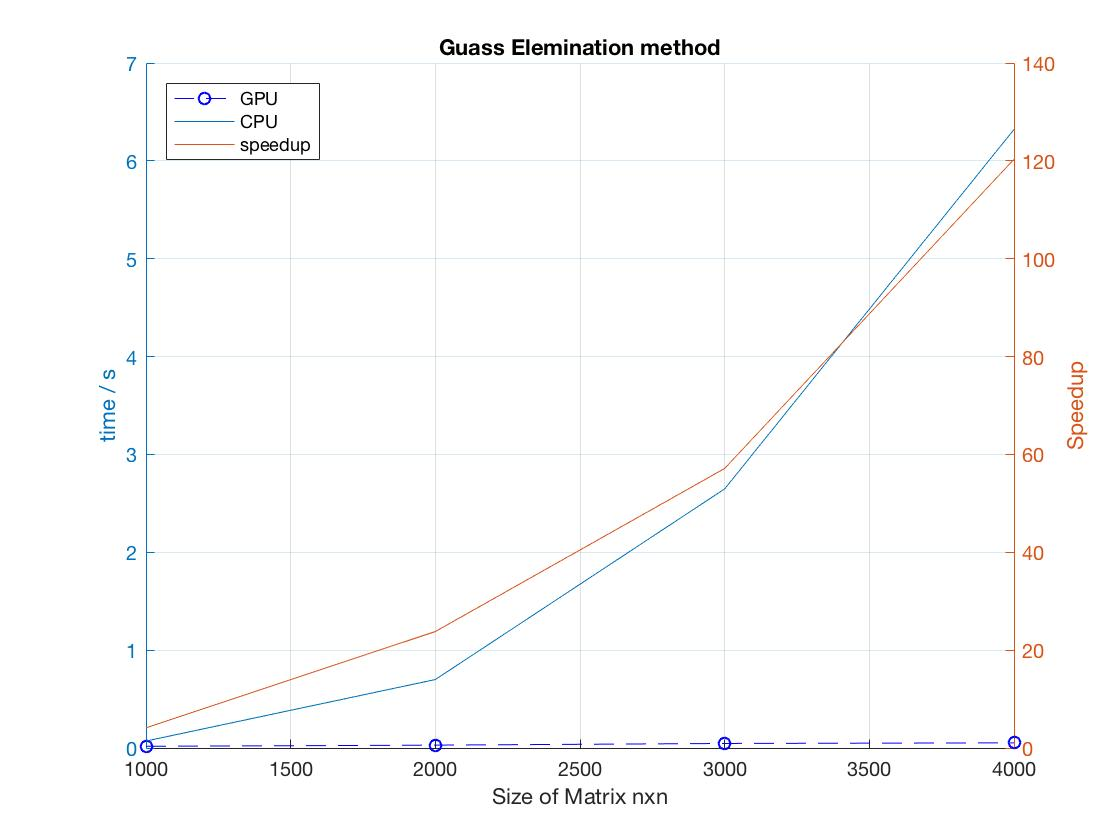
\includegraphics[width = 12cm]{Chapters/guass_elimination.jpg}
	\captionof{figure}{compare OCCA vs CPU performance }
\end{center}

As we can see CPU will more expensive than OCCA. We measure the length of matrix from 500X500 to 4000X4000. And GPU always take time near 0.xxx and CPU takes more time according to length of matrix. According to this conclusion, We can say that OCCA is better than CPU. 


\chapter{Jacobi method}
\section{Introduction}
Jacobi method is an iterative solver used for approximating the solution of diagonally dominant system of linear equations. 
The Jacobi method is easily derived by examining each of the n equations in the linear system Ax = b in isolation. If in the $i^{th}$ equation \\
\begin{equation}
	\sum^n_{j=1}a_{i,j}x_j = b_i
\end{equation}
We solve for the value of $x_i$ while assuming the other entries of x remain fixed, We obtain\\
\begin{equation}
	x_i = (b_i - \sum_{j\neq i}a_{i,j}x_j)/a_{i,i}
\end{equation}
This suggests an iterative method defined by \\
\begin{equation}
	x_i^{(k)} = (b_i - \sum_{j\neq i}a_{i,j}x_j^{(k-1})/a_{i,i}
\end{equation}

Which is the Jacobi method.

\section{C++ implementation}
The C++ implementation as below:
\begin{lstlisting}[language=C, caption=Jacobi method in C++]
	for (int k = 0; k < num_iter; k++) {
		for (int i = 0; i < n; i++ ) {
			float sum = 0;
			for (int j = 0; j < n; j++ ) {
				if ( j != i ) {
					sum += (a[i * (n + 1)+ j] * x[j]);
				}
			}
            x_new[i] = ((a[i * (n + 1) + n]) - sum ) / a[i + i * (n + 1)];
        }
		for (int i = 0; i < n; i++) {
			x[i] = x_new[i];
        }
	}
\end{lstlisting}
This is Jacobi method, Where first loop is count the number of iteration and another loop i,j are start from 0 to n which is the size of the matrix nXn. x is the initial guess vector and x\_new is result vector. And in the last loop, We copy the x\_new to x. It run again and again till k is not equal or bigger than number of iteration.
\section{OCCA implementation}
The OCCA implementation as below:
\begin{lstlisting}[language=C, caption=Jacobi method in OCCA]
	for (int i = 0; i < n; i++; @tile(16, @outer, @inner) ) {
		x_new[i] = a[i * (n + 1) + n];
		float sum =0;
		for (int j = 0; j < n; j++ ) {
			if ( j != i ) {
				sum += a[i + j * (n + 1)] * x[j];
            }
        }
         x_new[i] = ((a[i * (n + 1) + n]) - sum ) / a[i + i * (n + 1)];
        }
        for (int i = 0; i < n; i++; @tile(16, @outer, @inner){
    		x[i] = x_new[i];
    }
\end{lstlisting}
This is OCCA implementation of Jacobi method. It is same as CPU implementation but here we are using the fourth value for for loop. It is @tile(16, @outer, @inner), the tile tag, tiling for-loops as one and two dimensional sets of inner/outer loops. The tile(16) assign the working dimension. In this example it assign the working dimension is 16. 
\section{OCCA vs CPU}
\begin{center}
	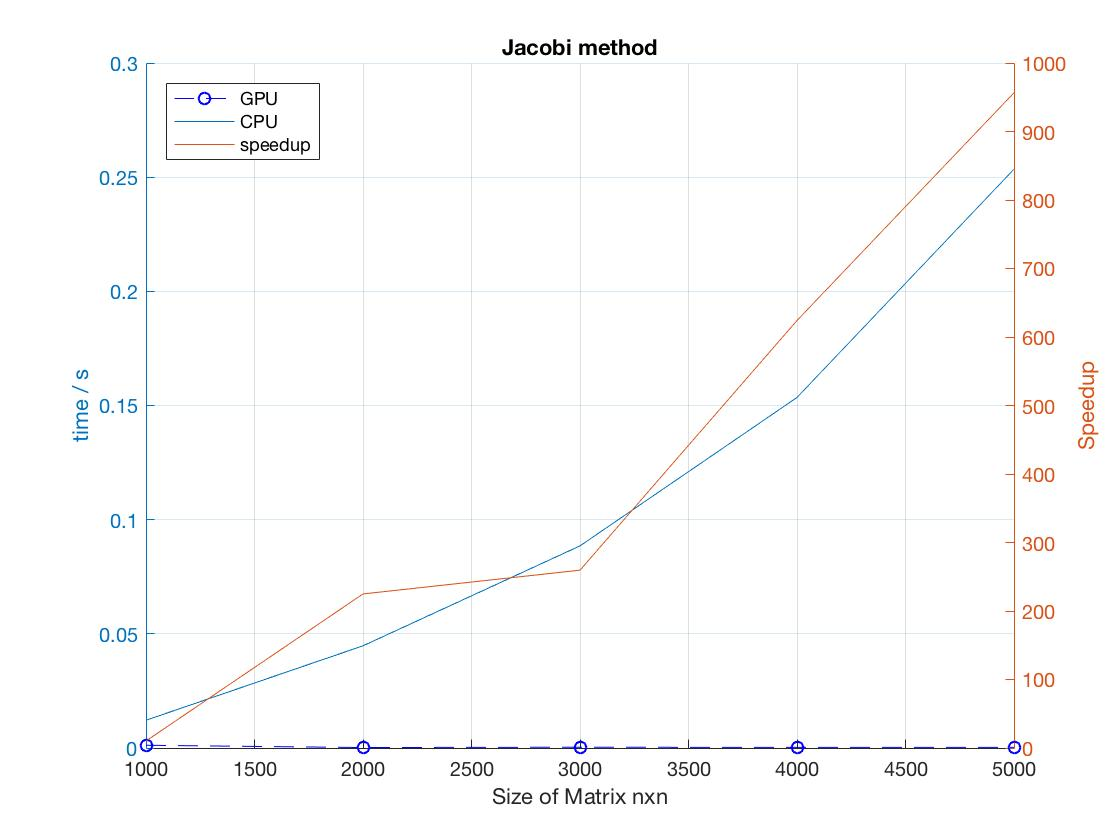
\includegraphics[width = 12cm]{Chapters/jacobi_method.jpg}
	\captionof{figure}{compare OCCA vs CPU performance }
\end{center}

For Jacobi method, OCCA is better than CPU. We can compare according to our results. We compare the matrix size from 1000X1000 to 5000X5000. In this size matrix, OCCA finish the program in 0.xxx time and CPU take time more than 0.2xx and it increase strictly according to size of the matrix. 